While there exists no application that cover all of the contextual and adaptive
features discussed in this paper, the following existing systems tackle many of
our ideas for a richer shell.

\subsection{xterm}
While there exists no application that covers all of the contextual and adaptive
features discussed in this paper, the following existing systems tackle many of
our ideas for a richer shell.
\begin{figure}[H]
  \centering
  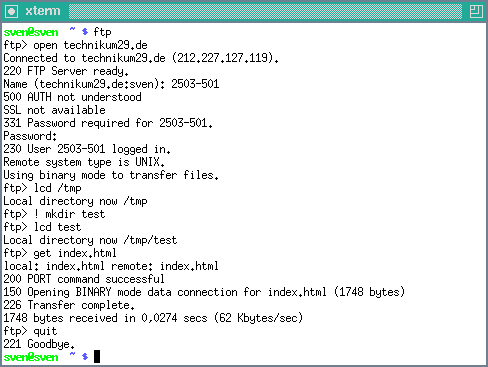
\includegraphics[width=0.8\linewidth]{figures/existing/xterm.png}
  \caption{An xterm window \cite{sven}.}
  \label{fig:xterm}
\end{figure}

\subsection{iterm2}
iterm2, like xterm, essentially just provides a terminal emulator, which in turn
provides a shell. However, it is able to provide far more contextual information
than that of xterm. The shell can alert the terminal emulator itself about the
state of the system (such as current git status), as well as embed images into
the text result.
\begin{figure}[H]
  \centering
  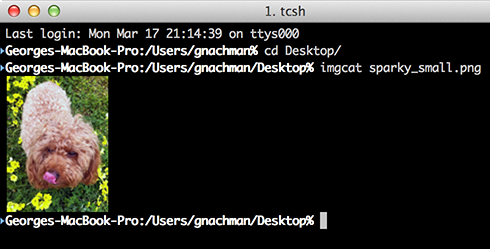
\includegraphics[width=0.8\linewidth]{figures/existing/iterm2.png}
  \caption{An iTerm 2 window, with inline images \cite{iterm}.}
  \label{fig:iterm}
\end{figure}

\subsection{zsh / Fish}
Both zsh and fish are shell programs designed to be more usable alternatives to
bash. A large part of this usability revolves around autocompletion and
suggestion. Fish will suggest command as you type (though it is not
bash-compatible). Zsh allows arbitrary autocompletion to be added to the system.
\begin{figure}[H]
  \centering
  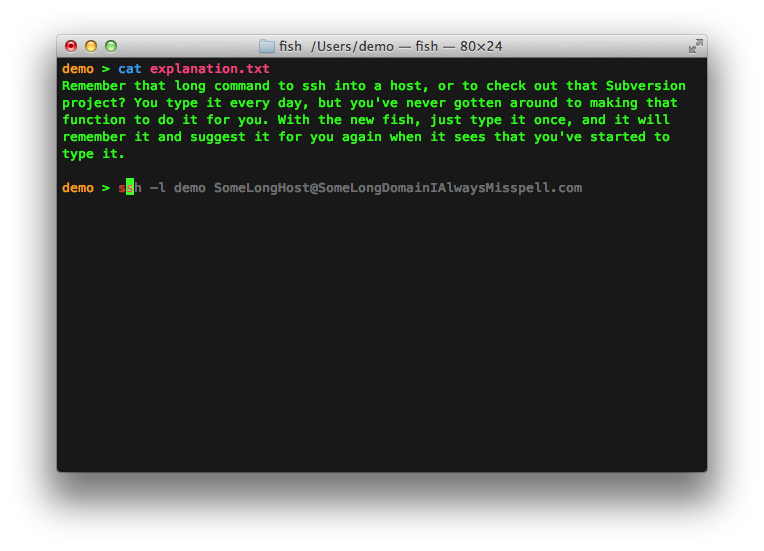
\includegraphics[width=0.8\linewidth]{figures/existing/fish.png}
  \caption{A fish shell, showing a suggested input \cite{fishshell}.}
  \label{fig:fish}
\end{figure}

\subsection{Explain Shell}
Explain shell is an educational tool which will break up a command, and explain
how it worked and what it means. This tool does not itself provide a shell, but
it does provide a tool which can be used to learn and understand bash and
related programs.
\begin{figure}[H]
  \centering
  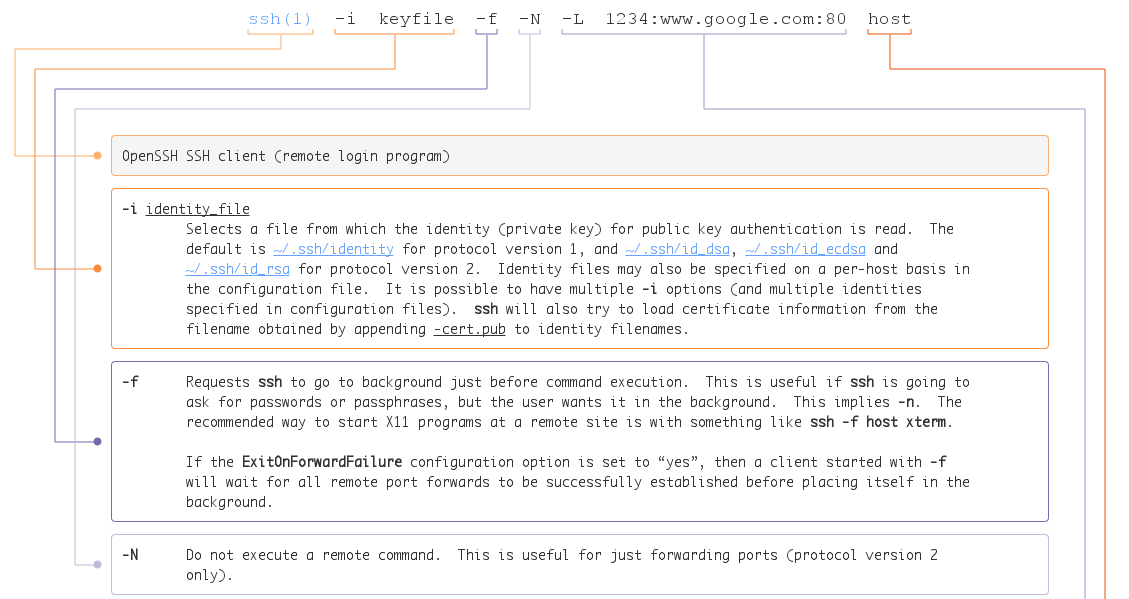
\includegraphics[width=0.8\linewidth]{figures/existing/eplainshell.png}
  \caption{A screen shot of explain shell breaking down a command \cite{explainshell}.}
  \label{fig:explainsh}
\end{figure}

\subsection{Jupyter}
Project jupyter is a modular, web based shell, designed for use with data
analytic languages (such as Julia, Python, and R). It allows graphical response
to commands, and let’s users distribute entire “sessions” of use. An important
feature is once a command is run, the user can edit the command. This chance
will then propagate through the history.

\begin{figure}[H]
  \centering
  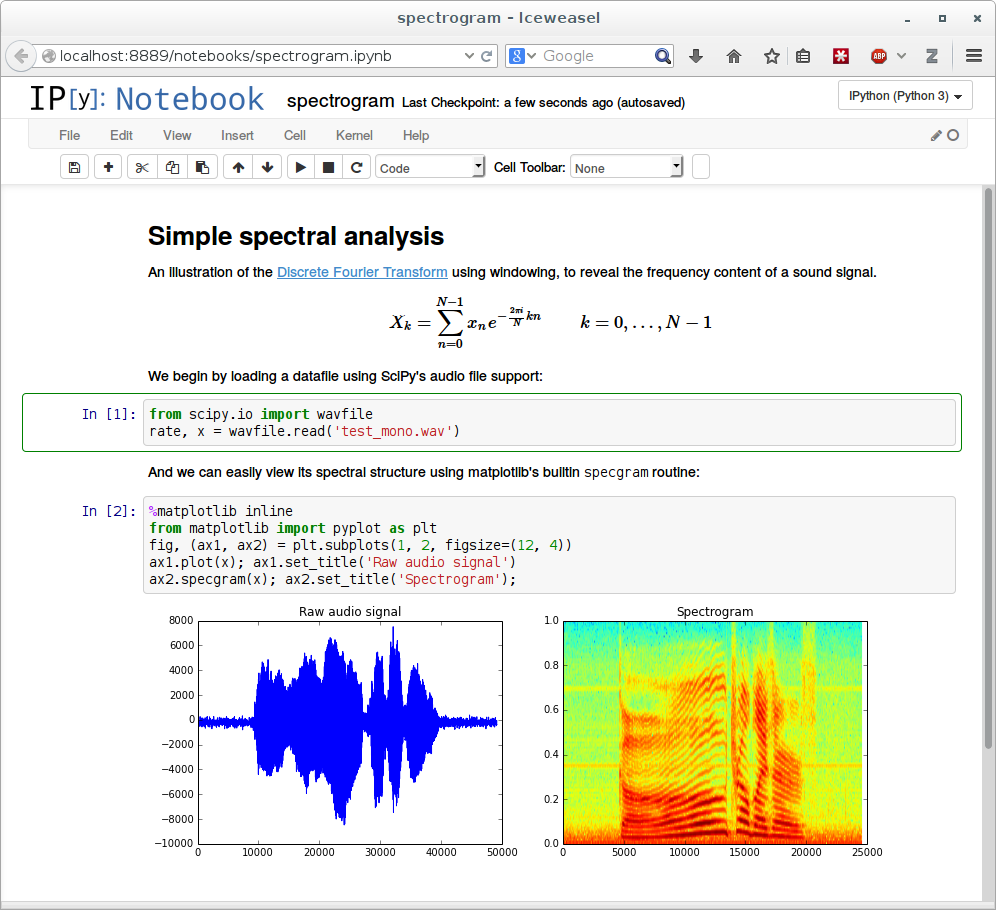
\includegraphics[width=0.8\linewidth]{figures/existing/ipython.png}
  \caption{An interactive jupyter session \cite{jupyter}.}
  \label{fig:jupyter}
\end{figure}

\subsection{Comparison of Features}

\begin{table}[H]
  \centering
  \begin{tabular}{|l|r|r|r|r|r|r|}
    \hline
    & This & \texttt{xterm} & iTerm 2 & \texttt{zsh}/\texttt{fish}
    & Explain Shell & Jupyter \\\hline
    Undo & V & X & X & X & X & V \\\hline
    File Actions & V & X & X & O & X & O\\\hline
    Automation Assistance & X & X & X & X & X & X\\\hline
    Command Results & V & X & X & X & V & O\\\hline
    Heads-Up Information & V & O & V & V & X & V\\\hline
  \end{tabular}
  \caption{Comparision of features. V -- able to perform the task, X -- unable
    to perform the task, O -- able to perform the task with poor interactive
    design.}
  \label{tab:features}
\end{table}
%%% Local Variables:
%%% mode: latex
%%% TeX-master: "documentation"
%%% End: